\documentclass{ximera}

\input{../../preamble.tex}

\author{Bobby Ramsey}

\begin{document}
\begin{exercise}

	% Find limit e^{-t} as t\to \infty
	Find the limits:
	\begin{align*}
		\lim_{t\to \infty} e^t &= \answer{\infty}\\
		\\
		\lim_{t \to -\infty} e^t &= \answer{0}\\
		\\
		\lim_{t\to \infty} e^{-t} &= \answer{0}\\
		\\
		\lim_{t \to -\infty} e^{-t} &= \answer{\infty}
	\end{align*}

	\begin{exercise}
	%setup logistic equation.  Find limit as $t\to \infty$
	A particular deer population has size given by:
	\[ P(t) = \frac{8000}{40+160e^{-0.1t}} \]
	with $t$ measured in years since 1990.
	What happens to the population size, as time goes on? (i.e. Find $\displaystyle \lim_{t\to\infty}P(t)$.)
		
	\[ \lim_{t\to\infty} P(t) = \answer{200} \]
	
		\begin{exercise}
		
			A graph of $P(t)$ is below.
			
			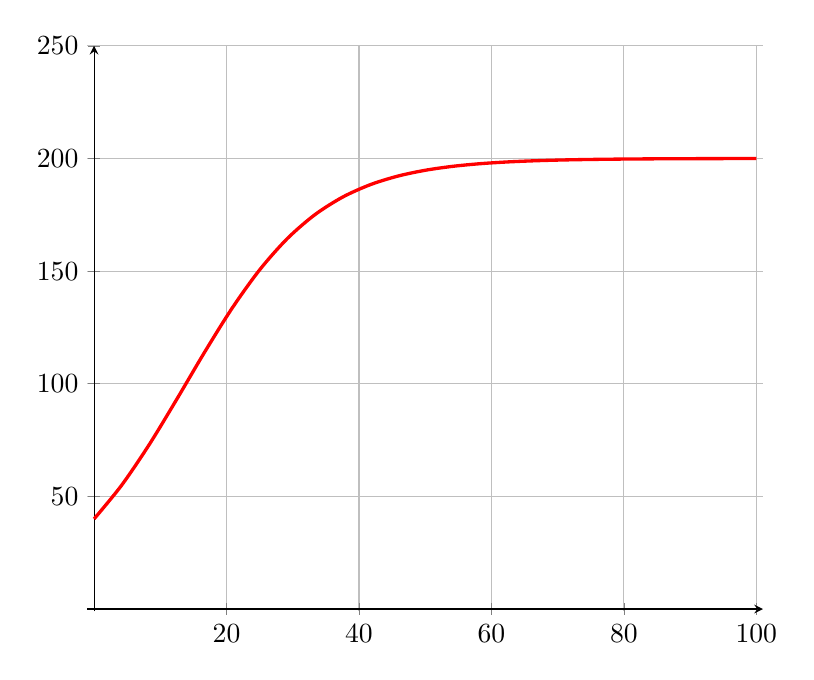
\begin{tikzpicture}
				\begin{axis}[
					xmin=-1, xmax=101, ymin=-1,ymax=250,    
					axis lines =middle, 
					every axis y label/.style={at=(current axis.above origin),anchor=south},
					every axis x label/.style={at=(current axis.right of origin),anchor=west},
					%xtick={0,...,100}, ytick={0,...,200},
					grid=major, width=4in,
					]
					\addplot[color=red, very thick, smooth, domain=0:100]{(8000)/(40+160*e^(-0.1*x))};
				\end{axis}
			\end{tikzpicture}

		% Find rate of change of population
		At what rate was the population changing in 2000? (Round to 1 decimal place)
		
		\[ \eval{ \ddt{P(t)} }_{t=10} = \answer{4.8} \text{ individuals / year } \]	
	
		\end{exercise}
	\end{exercise}


\end{exercise}
\end{document}